\documentclass[tikz,border=10pt]{standalone}
% Scale s = 0.014981 cm/px (from STYLE METRICS); origin at ink-bbox centre (303.5, 208.5) px
\usepackage{amsmath}
\begin{document}
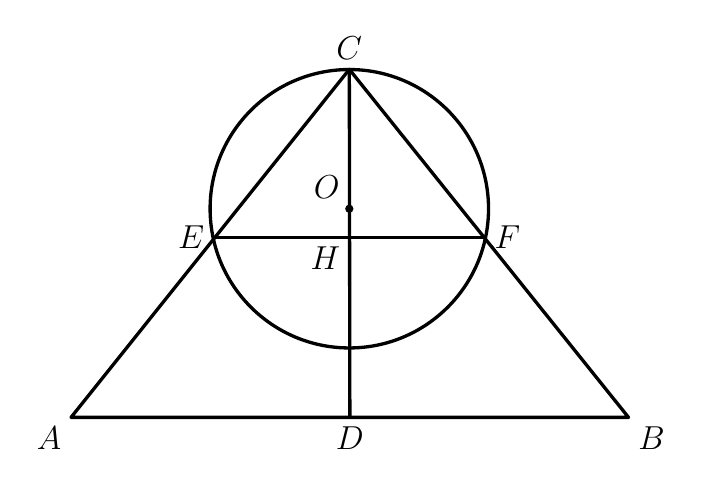
\begin{tikzpicture}[line join=round]
  % Named coordinates (converted from pixels, y flipped)
  \coordinate (A) at (-3.534,-2.285);
  \coordinate (B) at (3.546,-2.285);
  \coordinate (C) at (0,2.135);
  \coordinate (D) at (0.007,-2.285);
  \coordinate (O) at (0,0.365);
  \coordinate (H) at (0.007,0.007);
  \coordinate (E1) at (-1.720,0);   % chord left end (E)
  \coordinate (E2) at (1.720,0);    % chord right end (F)

  % Circle centred at O, same weight as the straight segments
  \draw[line width=1.2pt] (O) circle (1.768);

  % Triangle ABC
  \draw[line width=1.2pt] (A) -- (B) -- (C) -- cycle;

  % Vertical CD through O and H down to D
  \draw[line width=1.2pt] (C) -- (D);

  % Horizontal chord through H
  \draw[line width=1.2pt] (E1) -- (E2);

  % Filled dot at centre O
  \fill (O) circle (1.5pt);

  % Labels
  \node[below left] at (A) {\fontsize{12}{14.4}\selectfont $A$};
  \node[below right] at (B) {\fontsize{12}{14.4}\selectfont $B$};
  \node[above] at (C) {\fontsize{12}{14.4}\selectfont $C$};
  \node[below] at (D) {\fontsize{12}{14.4}\selectfont $D$};
  \node[above left] at (O) {\fontsize{12}{14.4}\selectfont $O$};
  \node[below left] at (H) {\fontsize{12}{14.4}\selectfont $H$};
  % E placed to the left of its point (east anchor, no upward offset)
  \node[anchor=east] at (E1) {\fontsize{12}{14.4}\selectfont $E$};
  \node[right] at (E2) {\fontsize{12}{14.4}\selectfont $F$};
\end{tikzpicture}
\end{document}